\chapter{Java-Programm}
\label{sec:java-programm}

\section{Anforderungen}
\subsection{Programm}
Die Hauptaufgabe des Programms ist es dem Benutzer eine Möglichkeit zum Steuern der Katzenfütterungsanlage zu Verfügung zu stellen. Weiters soll das Programm die Motoren steuern und die Sensoren in der Anlage auswerten können. Für diese Aufgabe sollen die IO-Pins am Raspberry verwendet werden.
\subsection{Design - Benutzerinterface}
Das Design der GUI-Fenster soll einfach und übersichtlich gestaltet werden. Auf der Hauptseite, also der Seite die immer zu sehen ist, sollen Informationen dargestellt werden, die dem Benutzer einen schnellen Überblick über den Zustand der Anlage geben. Alle anderen nicht direkt ersichtlichen Funktionen sollen über sinnvoll benamte Menüpunkte erreichbar sein.
Der Benutzer soll mit Hilfe eines kleinen Touchdisplays die Möglichkeit haben die Anlage zu steuern. Deswegen muss darauf geachtet werden, dass alle GUI-Fenster sinnvoll per Touch-Gesten verwenbar sind.
\subsection{Externe Steuerung}
Da die Katzenfütterungsanlage die Katze füttern soll, wenn die Familie der Katze auf Urlaub ist, sollte die Anlage auch über das Internet erreichbar sein. Dafür gibt es die Möglichkeit einen Benutzer auf der Anlage anzulegen mit welchem man anschließend über eine Webseite auf die Anlage zugreigen kann. 

\newpage

\section{Voruntersuchung}
\subsection{Wieso Java und nicht C?}
Zu Beginn musste entschieden werden mit welcher Programmiersprache gearbeitet werden soll. Zur Auswahl standen Java und C.
Vorteile von C:
\begin{itemize}
\item[1] Echtzeitfähige Steuerung der Motoren und Senosren
\item[2] Hardwarenahe Programmierung für die Pins
\end{itemize}
Vorteile von Java:
\begin{itemize}
\item[1] Erstellen einer GUI ist einfacher
\item[2] Implementieren eines Servers ist einfacher
\end{itemize}

Nach dem Gegenüberstellen der Vorteile wurde Java als Programmiersprache gewählt.

\subsection{Wieso das Raspberry Pi 3 Model B?}
Schon zu Beginn der Diplomarbeit war klar, dass mit deinem Raspberry gearbeitet werden soll. Nun musste entschieden werden welches Model verwendet werden soll. Wir haben das Raspberry Pi 3 Model B aufgrund folgender technischer Daten gewählt:
\begin{itemize}
\item[1] Rechenleistung
\item[2] Anzahl der GPIO-Pins
\item[3] WLAN-Fähigkeit
\end{itemize}

\subsection{Auswahl eines Touchdisplays}
Das Display muss folgendet Anforderungen erfüllen:
\begin{itemize}
\item[1] Es muss ein Touchscreen-Display sein
\item[2] Es muss einfach an das Raspberry anschließbar sein
\item[3] Es sollte nicht zu teuer sein
\end{itemize}

Aufgrund dieser Anforderungen wurde das Touchdisplay von Raspberry gewählt.

\subsection{Wieso pi4j?}
Da Java als Programmiersprache gewählt wurde, musste eine Möglichkeit die GPIO-Pins anzusteuern gefunden werden.
Da bei der Recherche außer pi4j Java kaum etwas gefunden wurde, wurde pi4j gewählt. Weiters vorteilhaft ist, dass das Ansteuern der Pins via Code nicht sehr kopliziert ist. 

\subsection{Wieso Mongodb?}
Eine Datenbank wurde gewählt, weil es gegebüber des Speichers der Daten in eine Datei mehrere Vorteile aufweist. 
\subsubsection{Vorteil gegenüber Daten in Datei speichern}
Vorteile einer Datenbank:
\begin{itemize}
\item[1] Keine Probleme mit Pfaden
\item[2] Daten sind alle in einem Punkt gespeichert und nicht im System verteilt
\item[3] Der benötigte Code für die Datenbank macht das Programm übersichtlicher
\end{itemize}
\subsubsection{Vergleich mit anderen Datenbanken}
Vorteile von Mongodb gegenüber anderen Datenbanken (zB mySQL):
\begin{itemize}
\item[1] Mongodb ist schemenlos (Daten benötigen keine bestimmte Struktur)
\item[2] Mongodb ist kostenfrei
\end{itemize}

\subsection{Kommunikation mit der Web-Applikation}
Der Server mit dem die Web-Applikation kommunizieren kann, wird aufgrund der gewählten Programmiersprache, in Java geschrieben. Der Server wird im Hintergrund aktiv sein und auf Anfragen der Web-Applikation warten. Je nach Anfrage wird der Server Daten zurück senden oder Methoden im Programm aufrufen. Die Daten, die bei der Kommunikation ausgetauscht werden, haben den Datentyp JSON.

\newpage

\section{Umsetzung}
Bei der Umsetzung, also beim Schreiben des Programms, wurde wie folgt vorgegangen. Zuerst wurden alle GUI-Fenster per Hand grob designed. Anschließend wurden diese im Netbeans als JFrame Form erstellt. Genaueres über die GUI-Fenster folgt uner Punkt 2.3.4. Danach wurden grundlegende Funktionen die das Programm zu erfüllen hat implementiert. Weiters wurden noch: Mongodb, pi4j, der Server und der ErrorAndWarningHandler als Singleton implementiert. 
\\ \\ 
Nun folgen ausführlichere Beschreibungen über die oben angeführten Klassen.

\subsection{Mongodb}
\subsubsection{Allgemeines}
Mongodb is ein schemenlose Datenbank. Schemenlos bedeuted, dass die Daten keine besondere Formatierung brauchen um gespeichert zu werden. Zusätzlich wird jedem gespeichertem Datensatz automatisch ein einmaliger Indentifikator gegeben. Weiters ist es kostenfrei und man benötigt keine Lizenzen.
\\
Bei einer schemenbehafteten Datenbank werden die Daten in Reihen und Spalten gegliedert. Um eine solche Datenbank effizient nutzen zu können wird auch ein einmaliger Identifikator.
\\ \\ 
In Mongodb sind Zeilen Collections und Spalten Documents. 
\\ \\
Die Datenbank kann in der Konsole mit dem Befehl \textbf{mongod} gestartet werden. In unserem konkreten Fall am Raspberry startet die Datenbank beim Starten des Raspberry automatisch. Weiters kann in der Konsole mit dem Befehl \textbf{mongo}, sofern die Datenbank gestartet ist, die Mongo-Shell geöffnet werden. In der Shell können alle angelegten Datebanken verwaltet werden. Unter verwalten wird das Ändern, Hinzufügen und Löschen von Daten verstanden. Es können auch neue Datenbanken angelegt oder alte Datenbanken gelöscht werden. 
\\ Befehle:
\begin{itemize}
\item[•] \textbf{show dbs} ... zeigt alle angelegten Datenbanken an
\item[•] \textbf{show collections} ... zeigt alle collections in einer Datebank
\item[•] \textbf{use} ... verwenden einer Datenbank, falls die Datenbank noch nicht existiert wird sie neu erstellt 
\\     (Beispiel: use <Datenbankname>)
\item[•] \textbf{drop()} ... löschen einer Datenbank
\\     (Beispiel: <Datenbankname>.drop() )
\item[•] \textbf{find()} ... suchen nach bestimmten Daten 
\\     (Beispiel: db.data.find() )
\item[•] \textbf{count()} ... zählt die Dokumente in einer Collection
\\     (Beispiel: db.<Collectionname>.count() )
\item[•] \textbf{insert()} ... hinzufügen eines Dokumentes
\\     (Beispiel: db.data.insert(\{"time1":"13:30"\})
\item[•] \textbf{updateOne()} ... updaten von Daten
\\     (Beispiel: db.data.updateOne(<DokumentID>, <Daten>) )
\item[•] \textbf{deleteOne()} ... löschen eins Dokumentes
\\     (Beispiel: db.data.deleteOne(<DokumentID>) )

\end{itemize}

\subsubsection{Datenbankmanagementsystem DBS}
Ein Datenbankmanagementsystem verwaltet eine oder mehrere Datenbanken. Mehrer Datenbanken werden dabei benötigt, wenn mehrere Anwenugen oder Programme jeweils eine eigene Datenbank brauchen. Ein Beispiel für ein DBS ist Mongodb.

\subsubsection{Singleton}
Der Datenbankzugriff wurde in einem Singleton implementiert. Dadurch wird nur ein Objekt der Datenbank erzeugt. Das bedeutet, dass nur von dieser Klasse aus auf die Datenbank zugegriffen wird und nur eine Verbindung geöffnet wird.
\\ Ein weiterer Vorteil davon ist, dass wenn einmal eine andere Datenbank verwendet werden sollte, nur diese eine Klasse geändert werden muss, weil nur in dieser Klasse der Code für die spezifische Datenbank enthalten ist.

\subsubsection{Code Beispiele}
Da am Raspberry die neueste Version von Mongodb nicht funktioniert, wird die Version 2.14.2 verwendet. Weitere Details zu diesem Thema sind unter Punkt 2.4.1 zu finden.
\\ Aus diesem Grund sind auch die Methoden, die als Beispiele angeführt sind, von der älteren Version. 
\\ \\ 
Als erstes muss eine Verbindung mit der Datenbank aufgebaut werden. Falls die Datenbank noch nicht existiert wird sie automatisch erstellt.
Dies ist in Java mit folgenden Methoden möglich:
\begin{lstlisting}[style=JavaStyle]
	MongoClient mongodb = new MongoClient();
	DB database = mongodb.getDB("<Datenbankname>");
\end{lstlisting}

Danach muss die Collection, in der gearbeitet werden soll, ausgewählt werden. Falls die Collection noch nicht existiert wird sie automatisch erstellt. Das ist mit der folgenden Methode möglich:
\begin{lstlisting}[style=JavaStyle]
	DBCollection coll = database.getCollection("<Collectionname>");
\end{lstlisting}
Anschließend kann mit der Datenbank gearbeitet werden. 
\begin{itemize}
\item[•] Die Dokumente in einer Collection zähle1n:
\begin{lstlisting}[style=JavaStyle]
	<Collectionname>.count();
\end{lstlisting}
\item[•] Ein Dokument aus der Datenbank lesen:
\begin{lstlisting}[style=JavaStyle]
	DBObject document = <Collectionname>.find(<Identifikator>).next();
\end{lstlisting}
\item[•] Ein Dokument zu einer Collection hinzufügen:
\begin{lstlisting}[style=JavaStyle]
	<Collectionname>.insert(document);
\end{lstlisting}	
\item[•] Ein Dokument in einer Collection updaten:
\begin{lstlisting}[style=JavaStyle]
	<Collectionname>.update(<Identifikator>, document);
\end{lstlisting}
\end{itemize}

\newpage

Ein konkretes Beispiel des Codes aus dem Programm für die Katzenfütterungsanlage sieht so aus:
\begin{lstlisting}[style=JavaStyle]
	DBObject document = collUser.find(
			new BasicDBObject("identifier", "User")).next();
\end{lstlisting}
Diese Zeile Code sucht in der Collection \textbf{collUser} nach dem Dokument mit dem Identifikator \textbf{new BasicDBObject(\grqq{}identifier\grqq{}, \grqq{}User\grqq{})}. Das gefundene Dokument wird dann der Varibale \textbf{document} zugewiesen. 


\subsection{pi4j}
\subsubsection{Allgemeines}
Pi4j ist eine freie Software, welche Bibliotheken zur Verfügung stellt, mit denen es möglich ist, von einem Java Programm, auf die IO-Pins eines Raspberrys zuzugreifen. Dabei kann ein GPIO-Pin als In- oder Ouput definiert werden. Wenn ein Pin als Output definiert wird, kann er den State High (+5V) oder Low (0V) haben. Mit einem Input Pin, können Signale gemessen werden. Das Ergebnis der Messung ist wieder High oder Low. Weiters ist es auch möglich einem Pin einen Listener zuzuweißen. Dieser Listener wartet bis auf diesem Pin ein Event auftritt und führt dann zum Beispiel eine Methode aus. 
\\ \\
Pi4j stellt eine Verbindung von der JVM (Java Virtuaul Machine) zu dem nativen System des Raspberys her. Dadurch wird es möglich von dem Programm auf die Pins zuzugreifen. Die folgende Grafik zeigt welche Bibliotheken dazu verwendetwerden.

\begin{wrapfigure}{l}{0.5\textwidth}
\vspace{-35pt}
  \begin{center}
    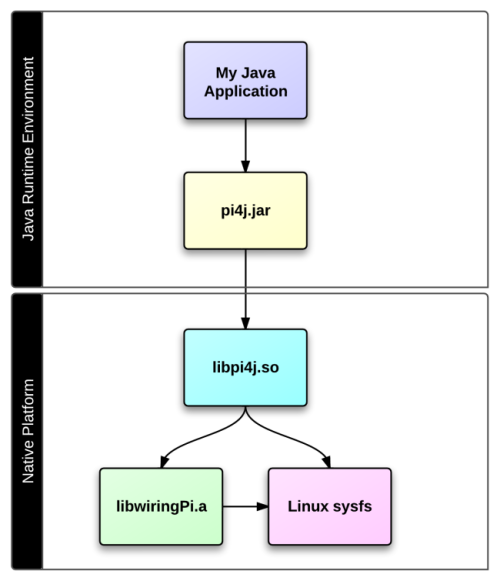
\includegraphics[width=0.45\textwidth]{Bilder/pi4j/dependencies}
  \end{center}
  \caption{Abhängigkeiten}
  \label{Magazin Vorne}
  \vspace{-170pt}
\end{wrapfigure}

Pi4j stellt eine Verbindung von der JVM (Java Virtuaul Machine) zu dem nativen System des Raspberys her. Dadurch wird es möglich von dem Programm auf die Pins zuzugreifen. Die folgende Grafik zeigt welche Bibliotheken dazu verwendetwerden.

\newpage

\subsubsection{Pin Numbering Sheme}

\begin{wrapfigure}{l}{0.5\textwidth}
\vspace{-40pt}
  \begin{center}
    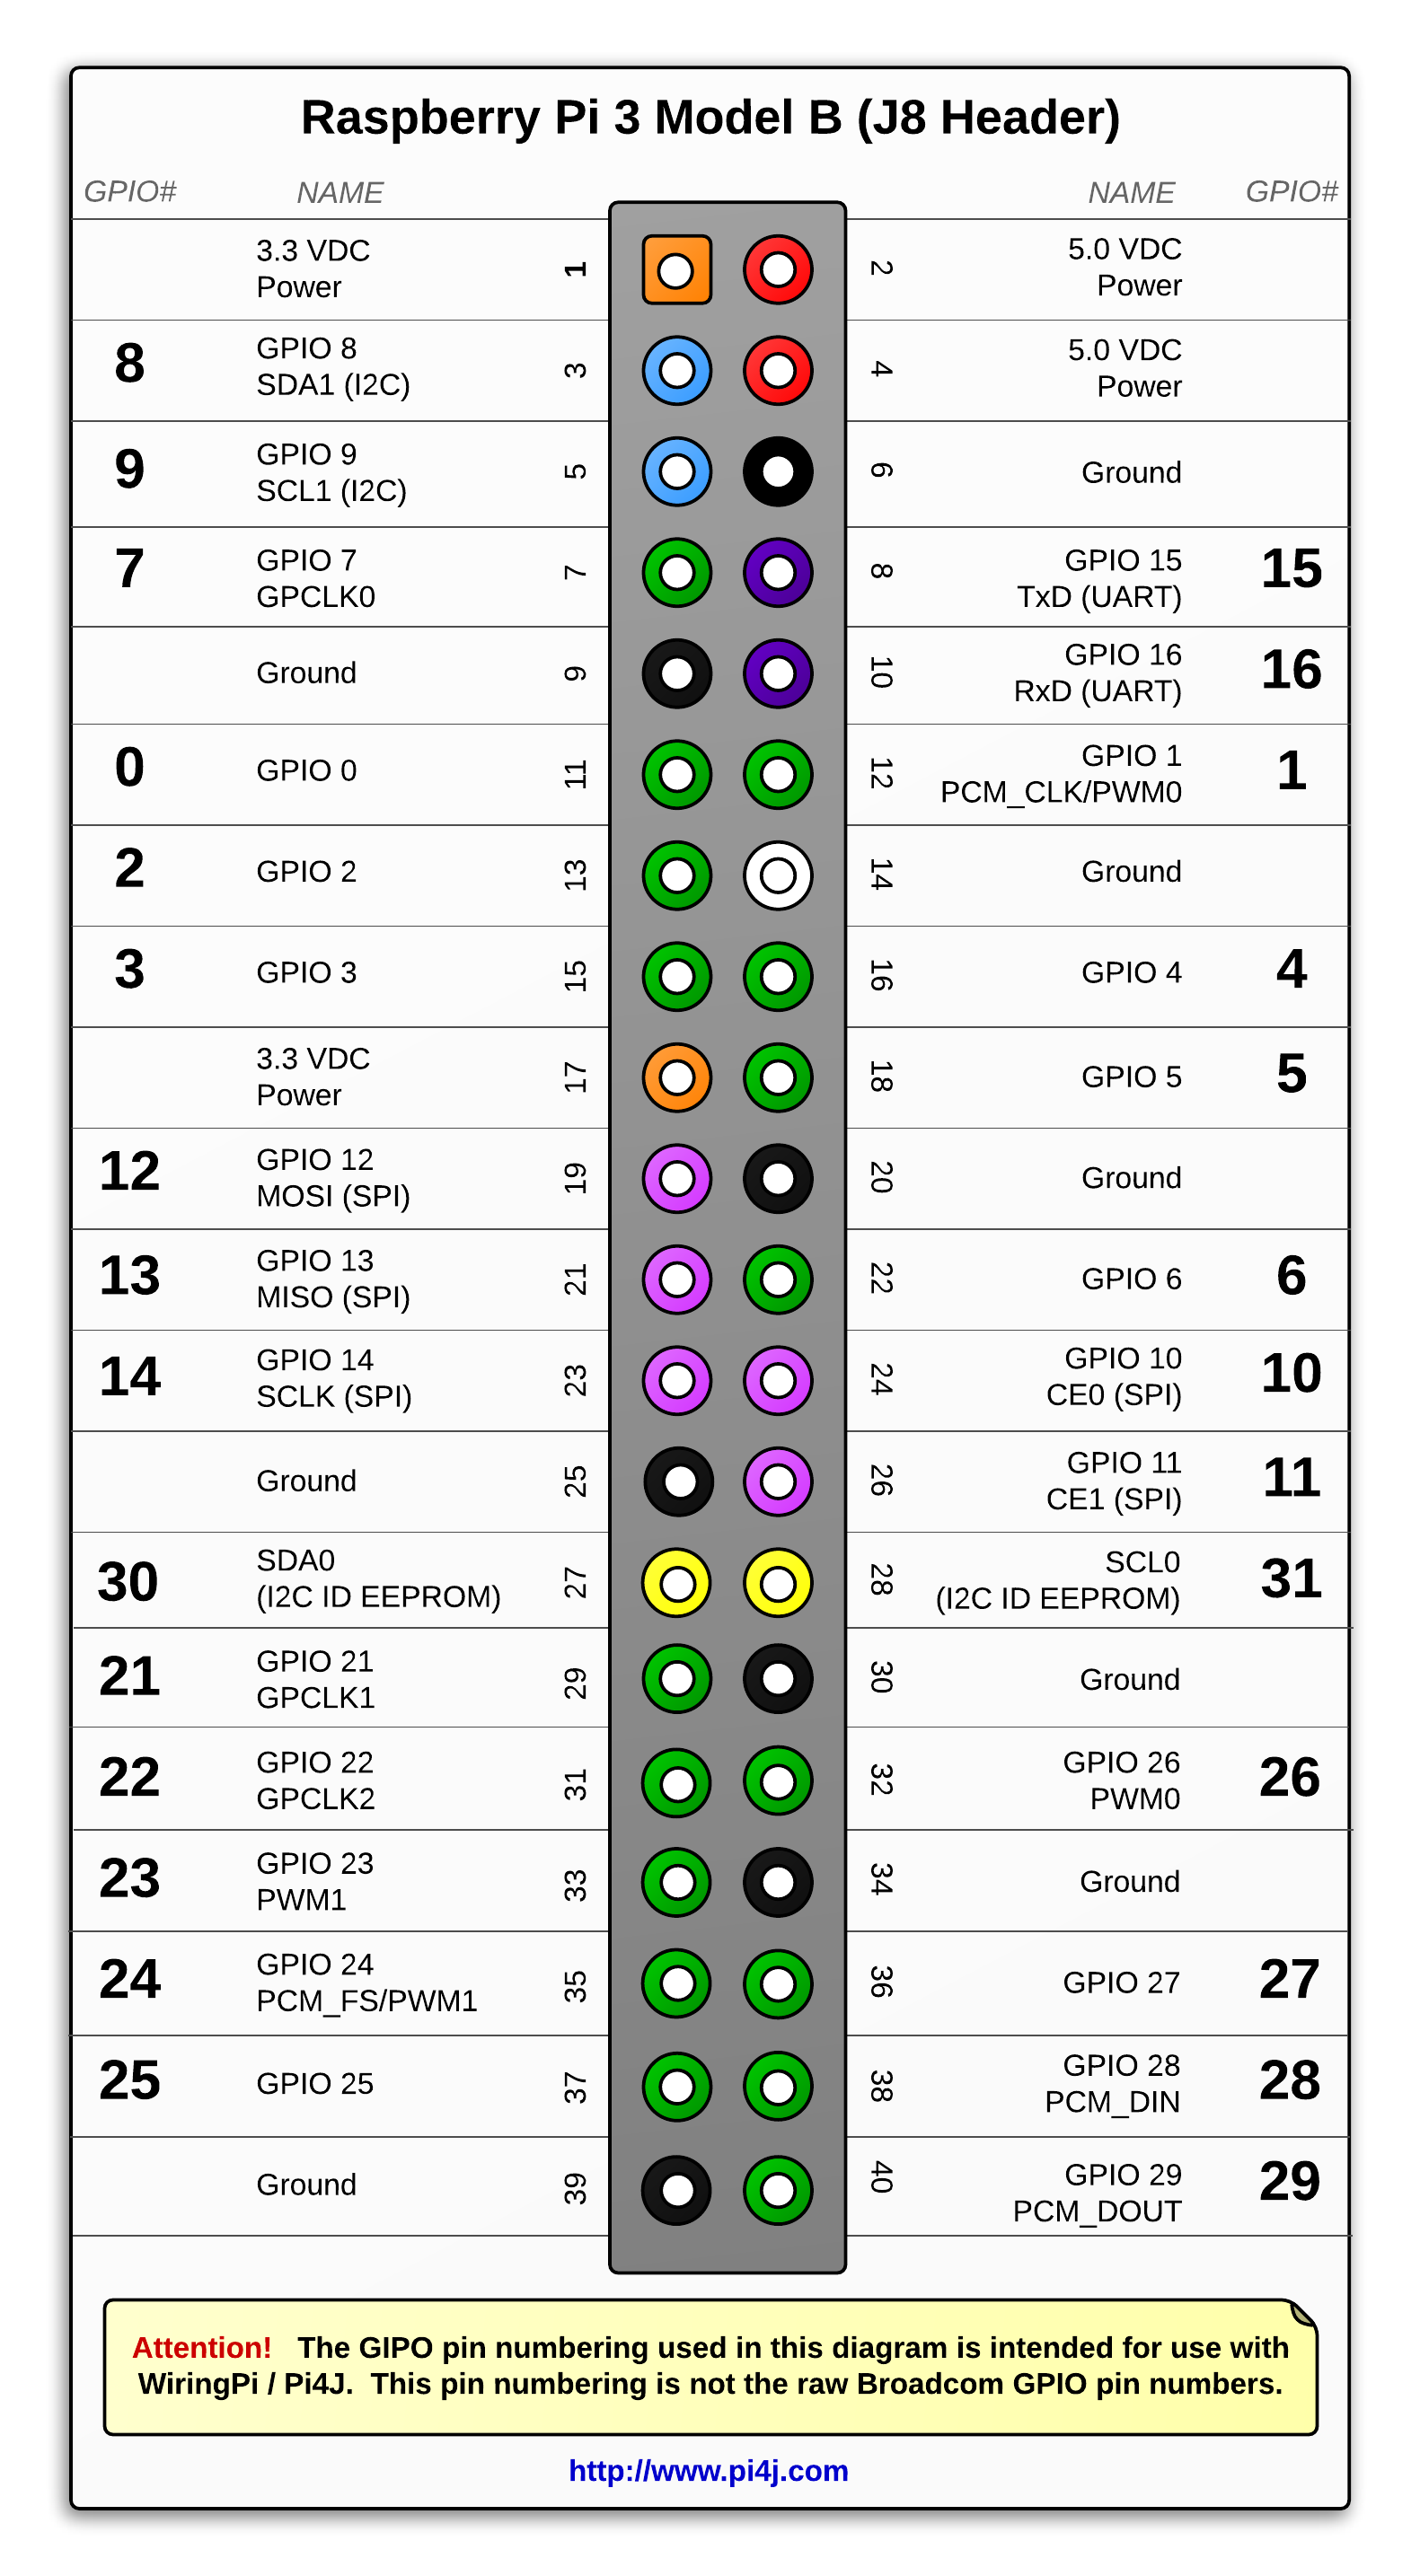
\includegraphics[width=0.50\textwidth]{Bilder/pi4j/PinNumberingSheme}
  \end{center}
  \caption{Pin Numbering Sheme}
  \label{Magazin Vorne}
  \vspace{-230pt}
\end{wrapfigure}

Am Raspberry haben einige Pins schon fest zugewiesene Funktionen, aber bei den GPIO-Pins kann der Programmierer selbst entscheiden, was der Pin sein soll.
\\ \\
In der Grafik ist zu sehen wie die Pins bei einem Raspberry Pi 3 \\ Model B belegt sind.

\subsubsection{Gewählte Pin Belegung}
Zum Ansteuern der Motoren und Auswerten der Sensoren wurden nur GPIO-Pins verwendet.

\subsubsection{Wieso Sigleton?}
\subsubsection{Code Beispiele}

\subsection{Server-Client}
\subsubsection{Übertragungsprotokoll}
\subsubsection{Wie wird geantwortet?}
\subsubsection{Was wird am Raspberry vom Java-Programm gemacht?}

\subsection{GUI-Fenster}
\subsubsection{MainWindow}
\subsubsection{TimeManagement}
\subsubsection{CreateUser}
\subsubsection{ManualControl}
\subsubsection{Positionsinformation}
\subsubsection{SystemInfo}
\subsubsection{Update}
\subsection{Errors und Warnungsverarbeitung}

\section{Zusammenfassung/Verbesserungsmöglichkeiten}
\subsection{Probleme mit Mongodb am Raspberry}
\subsection{GUI auf "Touchscreen-Design" abändern}
\subsection{Besser Benutzerverwaltung - Mehrere Benutzer anlegen}
\subsection{Selbst erstellbare Vorlagen in denen Zeiten gespeichert werden}
